\documentclass[11pt,a4paper]{article}
\usepackage[margin=21mm]{geometry}
\usepackage{amsmath,amssymb,booktabs,array}
\usepackage{tikz}
\usepackage[T1]{fontenc}
\usepackage{lmodern}
\usepackage{xcolor}
\usepackage{hyperref}
\hypersetup{colorlinks=true,linkcolor=blue,urlcolor=blue}
\setlength{\parindent}{0pt}
\setlength{\parskip}{6pt}
\newcommand{\DD}{V_{\mathrm{DD}}}
\newcommand{\GND}{\mathrm{GND}}
\newcommand{\N}[1]{\mathrm{N}(#1)}
\newcommand{\Pmos}[1]{\mathrm{P}(#1)}
\newcommand{\NM}[4]{%
  \coordinate (#1t) at (#2,{#3+.5});\coordinate (#1b) at (#2,{#3-.5});
  \draw (#1t)--(#2,{#3+.28})--({#2+.12},{#3+.28})--({#2+.12},{#3-.28})--(#2,{#3-.28})--(#1b);
  \draw ({#2-.14},{#3-.2})--({#2-.14},{#3+.2});
  \draw ({#2-.55},#3)--({#2-.14},#3);
  \node[anchor=east] at ({#2-.62},#3) {$#4$};}
\newcommand{\PM}[4]{%
  \coordinate (#1t) at (#2,{#3+.5});\coordinate (#1b) at (#2,{#3-.5});
  \draw (#1t)--(#2,{#3+.28})--({#2+.12},{#3+.28})--({#2+.12},{#3-.28})--(#2,{#3-.28})--(#1b);
  \draw ({#2-.14},{#3-.2})--({#2-.14},{#3+.2});
  \draw ({#2-.55},#3)--({#2-.35},#3);
  \draw ({#2-.295},#3) circle[radius=.055];
  \draw ({#2-.24},#3)--({#2-.14},#3);
  \node[anchor=east] at ({#2-.62},#3) {$#4$};}
\newcommand{\groundat}[2]{\draw (#1,#2)--(#1,{#2-.13});
  \draw ({#1-.28},{#2-.13})--({#1+.28},{#2-.13});
  \draw ({#1-.18},{#2-.22})--({#1+.18},{#2-.22});
  \draw ({#1-.08},{#2-.31})--({#1+.08},{#2-.31});}
\newcommand{\AOIcircuit}[5]{%
\begin{tikzpicture}[line width=.8pt,x=.9cm,y=.9cm]
  \PM{P1}{.8}{6.1}{#1}\PM{P2}{3.8}{6.55}{#2}\PM{P3}{3.8}{5.45}{#3}
  \PM{P4}{.8}{3.95}{#4}\PM{P5}{3.8}{3.95}{#5}
  \draw (.8,7.2)--(3.8,7.2);\draw (2.3,7.2)--(2.3,7.5) node[above] {$\DD$};
  \draw (P1t)--(.8,7.2);\draw (P2t)--(3.8,7.2);\draw (P2b)--(P3t);
  \draw (P1b)--(.8,4.8)--(3.8,4.8)--(P3b);
  \draw (P4t)--(.8,4.8);\draw (P5t)--(3.8,4.8);
  \draw (P4b)--(.8,3.2)--(3.8,3.2)--(P5b);
  \draw (3.8,3.2)--(5.1,3.2) node[right] {$f$};
  \fill (3.8,3.2) circle[radius=.05];
  \NM{N1}{.8}{2.4}{#1}\NM{N2}{0}{1}{#2}\NM{N3}{1.7}{1}{#3}
  \NM{N4}{3.8}{2.4}{#4}\NM{N5}{3.8}{1}{#5}
  \draw (N1t)--(.8,3.2);\draw (N4t)--(3.8,3.2);\draw (N4b)--(N5t);
  \draw (N1b)--(.8,1.7);\draw (0,1.7)--(1.7,1.7);
  \draw (N2t)--(0,1.7);\draw (N3t)--(1.7,1.7);
  \draw (N2b)--(0,.3)--(3.8,.3)--(N5b);\draw (N3b)--(1.7,.3);
  \groundat{2.3}{.3}
  \node[anchor=west,font=\small,text=gray] at (5.1,5.5) {PUN};
  \node[anchor=west,font=\small,text=gray] at (5.1,1.7) {PDN};
\end{tikzpicture}}

\begin{document}
\begin{center}
  {\Large\bfseries Introduction to VLSI Design}\par
  {\large Homework 1 --- Fall 2023}\par
  Independent solutions with reviewed reference submissions
\end{center}
\textbf{Circuit conventions.} A bubble marks a PMOS gate. All NMOS bodies connect
to GND and all PMOS bodies to $\DD$. Wires meeting at the shown common nodes are
connected. Series means AND of switch-enable conditions; parallel means OR.
Device sizes are unrestricted in this logic-design homework.

\section*{1(a). Static CMOS for an AOI function}
The printed prompt places a bar over the \emph{entire} expression:
\[
 \boxed{f(w,x,y,z)=\overline{w(x+y)+yz}.}
\]
This bar is easy to lose during PDF text extraction. The pull-down network (PDN)
must conduct exactly when $\bar f=w(x+y)+yz$ is 1. Therefore use
\[
 \bigl[\N{w}\text{ series }(\N{x}\parallel\N{y})\bigr]
 \parallel \bigl[\N{y}\text{ series }\N{z}\bigr].
\]
Replacing every series connection by parallel and every parallel connection by
series gives the complementary pull-up network (PUN):
\[
 [\Pmos{w}\parallel(\Pmos{x}\text{ series }\Pmos{y})]
 \text{ series }[\Pmos{y}\parallel\Pmos{z}].
\]
\begin{center}
 \AOIcircuit{w}{x}{y}{y}{z}\par
 \textbf{Figure 1.} The requested AOI gate: 5 NMOS + 5 PMOS.
\end{center}
The PUN conducts when $(\bar w+\bar x\bar y)(\bar y+\bar z)=f$.
The two networks are complementary for all 16 input combinations. The output
is already $f$; an extra inverter would produce the wrong polarity.

\newpage
\section*{1(b). Static CMOS for the minority function}
The requested function is
\[
 f(x,y,z)=\bar x\bar y+\bar x\bar z+\bar y\bar z.
\]
It is 1 exactly when at most one of $x,y,z$ is 1. Its complement is the
three-input majority function:
\[
 \bar f=xy+xz+yz=x(y+z)+yz.
\]
The second equality shares the transistor controlled by $x$. A factored
10-transistor implementation uses
\begin{align*}
 \text{PDN: }&[\N{x}\text{ series }(\N{y}\parallel\N{z})]
              \parallel[\N{y}\text{ series }\N{z}],\\
 \text{PUN: }&[\Pmos{x}\parallel(\Pmos{y}\text{ series }\Pmos{z})]
              \text{ series }[\Pmos{y}\parallel\Pmos{z}].
\end{align*}
\begin{center}
 \AOIcircuit{x}{y}{z}{y}{z}\par
 \textbf{Figure 2.} The minority gate: 5 NMOS + 5 PMOS.
\end{center}
No complemented input wires are needed: a PMOS controlled by $x$ turns on
when $x=0$. Thus both parts of Question 1 use only true input literals,
as the prompt requires.

\begin{center}
\begin{tabular}{cccc@{\qquad}cccc}
\toprule
$x$&$y$&$z$&$f$&$x$&$y$&$z$&$f$\\\midrule
0&0&0&1&1&0&0&1\\
0&0&1&1&1&0&1&0\\
0&1&0&1&1&1&0&0\\
0&1&1&0&1&1&1&0\\\bottomrule
\end{tabular}
\end{center}

\newpage
\section*{2. Four-output controlled rotation}
Each legal control word has exactly one 0. Use 4 CMOS transmission gates
(TGs) at each output, one for each possible data source. If $c_i=0$, turn on
the corresponding TG using NMOS gate $\bar c_i$ and PMOS gate $c_i$.

Reading the original table in the stated order $c_3,c_2,c_1,c_0$ gives
\begin{align*}
 z_3&=\bar c_3a_3+\bar c_2a_2+\bar c_1a_1+\bar c_0a_0,\\
 z_2&=\bar c_3a_2+\bar c_2a_1+\bar c_1a_0+\bar c_0a_3,\\
 z_1&=\bar c_3a_1+\bar c_2a_0+\bar c_1a_3+\bar c_0a_2,\\
 z_0&=\bar c_3a_0+\bar c_2a_3+\bar c_1a_2+\bar c_0a_1.
\end{align*}
These equations describe the valid control words. In compact form,
$z_j=\sum_{k=0}^{3}\bar c_{3-k}a_{(j-k)\bmod4}$.

\begin{center}
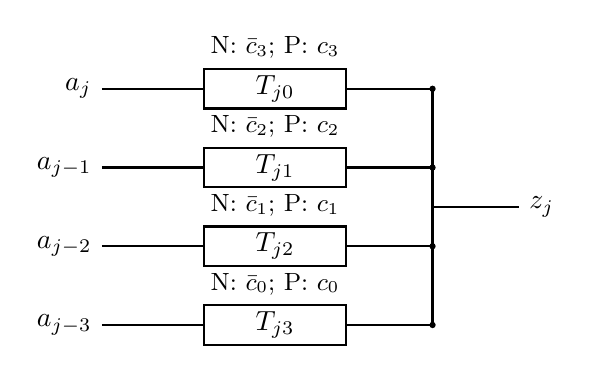
\begin{tikzpicture}[line width=.8pt,x=1cm,y=1cm]
 \foreach \y/\label/\control/\k in {4/{a_j}/3/0,3/{a_{j-1}}/2/1,2/{a_{j-2}}/1/2,1/{a_{j-3}}/0/3}{
   \node[anchor=east] at (0,\y) {$\label$};
   \draw (0,\y)--(1.3,\y);
   \draw (1.3,{\y-.25}) rectangle (3.1,{\y+.25});
   \node at (2.2,\y) {$T_{j\k}$};
   \node[font=\small] at (2.2,{\y+.52}) {N: $\bar c_{\control}$; P: $c_{\control}$};
   \draw (3.1,\y)--(4.2,\y);
   \fill (4.2,\y) circle[radius=.04];
 }
 \draw (4.2,1)--(4.2,4);
 \draw (4.2,2.5)--(5.3,2.5) node[right] {$z_j$};
\end{tikzpicture}\par
\textbf{Figure 3.} One output bank; build four copies for $j=0,1,2,3$.
\end{center}
All data subscripts in Figure 3 are modulo 4. The following table lists every
data-to-output connection, so the diagram specifies all 16 TGs:
\begin{center}
\begin{tabular}{c cccc}
\toprule
Output&$c_3=0$&$c_2=0$&$c_1=0$&$c_0=0$\\\midrule
$z_3$&$a_3$&$a_2$&$a_1$&$a_0$\\
$z_2$&$a_2$&$a_1$&$a_0$&$a_3$\\
$z_1$&$a_1$&$a_0$&$a_3$&$a_2$\\
$z_0$&$a_0$&$a_3$&$a_2$&$a_1$\\\bottomrule
\end{tabular}
\end{center}

\newpage
\section*{2. Transmission-gate transistor implementation}
\begin{center}
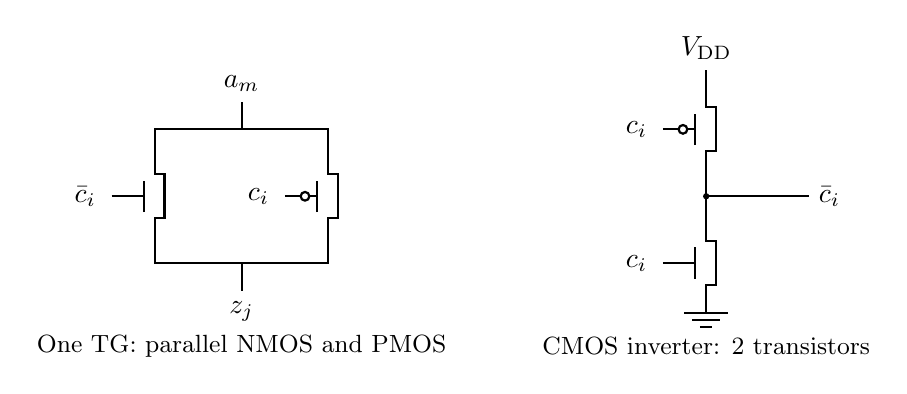
\begin{tikzpicture}[line width=.8pt,x=1cm,y=1cm]
 \NM{TN}{0}{0}{\bar c_i}\PM{TP}{2.2}{0}{c_i}
 \draw (TNt)--(0,.85)--(2.2,.85)--(TPt);
 \draw (TNb)--(0,-.85)--(2.2,-.85)--(TPb);
 \draw (1.1,.85)--(1.1,1.2) node[above] {$a_m$};
 \draw (1.1,-.85)--(1.1,-1.2) node[below] {$z_j$};
 \node[font=\small] at (1.1,-1.9) {One TG: parallel NMOS and PMOS};
 \begin{scope}[xshift=7cm]
   \PM{IP}{0}{.85}{c_i}\NM{IN}{0}{-.85}{c_i}
   \draw (IPt)--(0,1.6) node[above] {$\DD$};
   \draw (IPb)--(INt);\draw (0,0)--(1.3,0) node[right] {$\bar c_i$};
   \fill (0,0) circle[radius=.04];\groundat{0}{-1.35}
   \node[font=\small] at (0,-1.9) {CMOS inverter: 2 transistors};
 \end{scope}
\end{tikzpicture}\par
\textbf{Figure 4.} Expanded TG and its complementary-control generator.
\end{center}
For each $i=0,1,2,3$, generate $\bar c_i$ with one shared CMOS inverter.
When $c_i=0$, both TG transistors conduct. When $c_i=1$, both are off.
The NMOS passes a strong 0 and the PMOS passes a strong 1, giving a full-swing
static connection to the selected data input.

The total is
\[
 4\text{ outputs}\times4\text{ TGs}\times2\text{ MOSFETs}
 +4\text{ inverters}\times2\text{ MOSFETs}
 =\boxed{40\text{ transistors}.}
\]
The four control inverters serve all output banks. Under a legal control word,
each output is connected to exactly one data input. No weak NMOS-only pass-high
path and no data-to-data contention exists in these settled legal states.

\textbf{Control-domain assumption.} The problem specifies only 0111, 1011,
1101 and 1110. This design assumes those stable one-low words. For 1111 the
outputs float; with several controls low, several data inputs may be shorted
together. These omitted control cases are not assigned an output value by the
prompt. A separate decoder would be required if operation outside the four
specified states were also required. The verification script characterizes
all omitted control combinations without claiming that they satisfy an
unstated specification.

\textbf{Reproducible connectivity.} In \texttt{circuits.json},
\texttt{TjkN} and \texttt{TjkP} connect $a_{(j-k)\bmod4}$ to $z_j$.
Their gates are respectively $\bar c_{3-k}$ and $c_{3-k}$, exactly as in
Figures 3 and 4. The four inverter pairs are also listed explicitly.

\newpage
\section*{3(a). Function of the pass-transistor circuit}
The upper NMOS is enabled by $A$ and passes $\bar B$. The lower NMOS is
enabled by $\bar A$ and passes $B$. Thus
\[
 F=\begin{cases}B,&A=0,\\\bar B,&A=1,\end{cases}
 \qquad\boxed{F=A\bar B+\bar AB=A\oplus B.}
\]
\begin{center}
\begin{tabular}{cccl}\toprule
$A$&$B$&$F$&Enabled path\\\midrule
0&0&0&Lower transistor passes $B$\\
0&1&1&Lower transistor passes $B$\\
1&0&1&Upper transistor passes $\bar B$\\
1&1&0&Upper transistor passes $\bar B$\\\bottomrule
\end{tabular}
\end{center}
This Boolean interpretation does not claim that an NMOS alone passes an
ideal rail-level 1; its high voltage can be degraded by the threshold voltage.

\section*{3(b). Full-swing static CMOS XOR}
For a complementary static CMOS replacement,
$\bar F=AB+\bar A\bar B$. Put these two two-transistor series branches in
parallel in the PDN. The dual PUN consists of two parallel pairs in series.
Generate $\bar A$ and $\bar B$ with two copies of the CMOS inverter in Figure 4.

\begin{center}
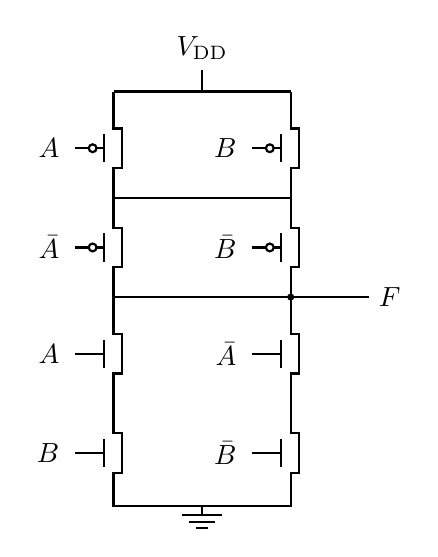
\begin{tikzpicture}[line width=.8pt,x=.9cm,y=.9cm]
 \PM{XP1}{.7}{5.2}{A}\PM{XP2}{3.2}{5.2}{B}
 \PM{XP3}{.7}{3.8}{\bar A}\PM{XP4}{3.2}{3.8}{\bar B}
 \draw (.7,6)--(3.2,6);\draw (1.95,6)--(1.95,6.3) node[above] {$\DD$};
 \draw (XP1t)--(.7,6);\draw (XP2t)--(3.2,6);
 \draw (XP1b)--(.7,4.5)--(3.2,4.5)--(XP2b);
 \draw (XP3t)--(.7,4.5);\draw (XP4t)--(3.2,4.5);
 \draw (XP3b)--(.7,3.1)--(3.2,3.1)--(XP4b);
 \draw (3.2,3.1)--(4.3,3.1) node[right] {$F$};\fill (3.2,3.1) circle[radius=.05];
 \NM{XN1}{.7}{2.3}{A}\NM{XN2}{.7}{.9}{B}
 \NM{XN3}{3.2}{2.3}{\bar A}\NM{XN4}{3.2}{.9}{\bar B}
 \draw (XN1t)--(.7,3.1);\draw (XN3t)--(3.2,3.1);
 \draw (XN1b)--(XN2t);\draw (XN3b)--(XN4t);
 \draw (XN2b)--(.7,.15)--(3.2,.15)--(XN4b);\groundat{1.95}{.15}
\end{tikzpicture}\par
\textbf{Figure 5.} XOR core: 4 NMOS + 4 PMOS, plus two input inverters.
\end{center}
PUN enable is $(\bar A+\bar B)(A+B)=A\bar B+\bar AB$.
Total transistor count, including the input inverters, is $8+4=\boxed{12}$.

\newpage
\section*{Verification and comparison with supplied answers}
Run \texttt{python check\_logic.py}. The checker evaluates independently
specified Boolean formulas and table entries, then determines actual outputs
by graph reachability through enabled MOS switches. It does not substitute
the expected output into a network model.

\begin{center}
\begin{tabular}{lrr}\toprule
Circuit&Input cases&Output checks\\\midrule
Question 1(a)&16&16\\
Question 1(b)&8&8\\
Question 3 (including input inverters)&4&4\\
Question 2 (4 legal controls $\times$ 16 data words)&64&256\\\midrule
Total&&284\\\bottomrule
\end{tabular}
\end{center}
\textbf{Result: all 284 functional output checks pass.} For each static CMOS
case the output reaches exactly one supply rail, so there is neither a floating
output nor a direct rail short in the ideal-switch model. Every legal TG output
reaches exactly the required data input. The script also records 768 output
characterizations across the omitted control cases. This homework contains no
SPICE timing or sizing requirement; these checks do not establish analog
voltage margins, delay or power.

\begin{center}
\begin{tabular}{p{.21\linewidth}p{.70\linewidth}}\toprule
Supplied reference&Review and final integration\\\midrule
109501570, HW1&Correct AOI polarity and XOR. Its 12-transistor minority
gate is valid; the factored 10-transistor network is used here. Its encoded
two-level TG rotation is replaced by the directly controlled bank.\\[4pt]
110501512, HW1&Its Q1 transistor networks and directly controlled TG bank
provide useful topology checks. The minority-function algebra is rewritten
from the prompt. Its XOR core assumes complements; the final solution adds
explicit CMOS complement generators.\\[4pt]
110501558, HW1&Its photographed Q1(a) includes an extra output inverter,
which implements the positive AO expression rather than the printed AOI
function. Its minority and XOR ideas are consistent with the requested
functions; the final diagrams use the factored network and explicit
complement generators.\\\bottomrule
\end{tabular}
\end{center}
All three supplied submissions were reviewed visually, including handwritten
figures. The final equations, diagrams and connectivity model were derived
independently and cross-checked against those submissions. The original
assignment is preserved at
\href{../assignments/homework1.pdf}{\texttt{2023/assignments/homework1.pdf}}.
The retained and corrected reference claims are explained in
\texttt{REFERENCE\_COMPARISON.md}.

\textbf{Generated evidence.} \texttt{truth\_tables.csv} contains all 28 logic
rows; \texttt{mux\_connectivity.csv} contains the 256 legal output checks;
\texttt{illegal\_controls.csv} records the unspecified control cases;
\texttt{verification.json} summarizes the results;
\texttt{circuits.json} lists every checked transistor connection.
\end{document}
